%%%%%%%%%%%%%%%%%%%%%%%%%%%%%%%%%%%%%%%%%%%%%%%%%%%%%%%%%%%%%%%%%%%%%%
% LaTeX Template: Curriculum Vitae
%
% Source: http://www.howtotex.com/
% Feel free to distribute this template, but please keep the
% referal to HowToTeX.com.
% Date: July 2011
% 
%%%%%%%%%%%%%%%%%%%%%%%%%%%%%%%%%%%%%%%%%%%%%%%%%%%%%%%%%%%%%%%%%%%%%%
% How to use writeLaTeX: 
%
% You edit the source code here on the left, and the preview on the
% right shows you the result within a few seconds.
%
% Bookmark this page and share the URL with your co-authors. They can
% edit at the same time!
%
% You can upload figures, bibliographies, custom classes and
% styles using the files menu.
%
% If you're new to LaTeX, the wikibook is a great place to start:
% http://en.wikibooks.org/wiki/LaTeX
%
%%%%%%%%%%%%%%%%%%%%%%%%%%%%%%%%%%%%%%%%%%%%%%%%%%%%%%%%%%%%%%%%%%%%%%
\documentclass[paper=a4,fontsize=11pt]{article} % KOMA-article class
							
\usepackage[english]{babel}
\usepackage[utf8x]{inputenc}
\usepackage[protrusion=true,expansion=true]{microtype}
\usepackage{amsmath,amsfonts,amsthm}     % Math packages
\usepackage{graphicx}                    % Enable pdflatex
\usepackage[svgnames]{xcolor}            % Colors by their 'svgnames'
\usepackage[margin=1in]{geometry}        % Decrease margins to 1 inch to make CV wider%	\textheight=700px                    % Saving trees ;-)
\usepackage{url}

\usepackage[hidelinks]{hyperref}
\usepackage{geometry}
\usepackage{pdfpages}  % Permite adjuntar pdfs al final del documento
\usepackage{wrapfig}
\usepackage{lscape}
\usepackage{rotating}
\usepackage{epstopdf}
\usepackage{textcomp} % hace falta para poner apostrofe
%\usepackage[table]{xcolor} % para las tablas bonitas coloreadas. loads also »colortbl«
\usepackage{array} % necesario para formatear del tiron una columna de una tabla
\usepackage{booktabs}
%\usepackage{pbox} % necesario para introducir salto de linea en celdas de una tabla
\usepackage{longtable}
\usepackage{pdflscape}
\usepackage{amsmath}
\newcommand\T{\textrm{T}}  % "true"
\newcommand\F{\textrm{F}}  % "false"
\usepackage{xspace}

\usepackage{fancyhdr}
 
\pagestyle{fancy}
\fancyhf{}
\lhead{\textbf{Antonio Ortega Jiménez}}
\rhead{\textit{Curriculum Vitae}}
\rfoot{Page \thepage\xspace of 3}

\fancypagestyle{plain}{%
  \fancyhf{}% Clear header/footer
  \fancyfoot[OR]{Page \thepage\xspace of 3}%
  \fancyfoot[EL]{Page \thepage\xspace of 3}%
  \renewcommand{\headrulewidth}{0pt}%
}


\def\changemargin#1#2{\list{}{\rightmargin#2\leftmargin#1}\item[]}
\let\endchangemargin=\endlist  %change the margins as given by arguments

%% Font usage
%%% ------------------------------------------------------------
\usepackage[T1]{fontenc}
\usepackage[osf]{mathpazo}



\frenchspacing              % Better looking spacings after periods
\pagestyle{empty}           % No pagenumbers/headers/footers


	
%%% Macros
%%% ------------------------------------------------------------
\newlength{\spacebox}
\settowidth{\spacebox}{8888888888}			% Box to align text
\newcommand{\sepspace}{\vspace*{1em}}		% Vertical space macro

\newcommand{\MyName}[1]{ % Name
		\Huge \usefont{OT1}{phv}{b}{n} \hfill #1
		\par \normalsize \normalfont}
		
\newcommand{\MySlogan}[1]{ % Slogan (optional)
		\large \usefont{OT1}{phv}{m}{n}\hfill \textit{#1}
		\par \normalsize \normalfont}

\newcommand{\NewPart}[1]{\section*{
									%\uppercase
									{#1}}}

\newcommand{\PersonalEntry}[2]{
		\noindent\hangindent=2em\hangafter=0 % Indentation
		\parbox{\spacebox}{        % Box to align text
		\textit{#1}}		       % Entry name (birth, address, etc.)
		\hspace{1.5em} #2 \par}    % Entry value

\newcommand{\SkillsEntry}[2]{      % Same as \PersonalEntry
		\noindent\hangindent=2em\hangafter=0 % Indentation
		\parbox{\spacebox}{        % Box to align text
		\textit{#1}}			   % Entry name (birth, address, etc.)
		\hspace{1.5em} #2 \par}    % Entry value	
		
\newcommand{\EducationEntry}[4]{
		\noindent \textbf{#1} \hfill      % Study
		\colorbox{Black}{%
			\parbox{6em}{%
			\hfill\color{White}#2}} \par  % Duration
		\noindent \textit{#3} \par        % School
		\noindent\hangindent=1em\hangafter=0 \small \begin{changemargin}{2em}{3cm}#4 \end{changemargin} % Description
		\normalsize \par}

\newcommand{\AwardEntry}[4]{
		\noindent \textbf{#1} \hfill      % Study
		\colorbox{Black}{%
			\parbox{3em}{%
			\hfill\color{White}#2}} \par  % Duration
		\noindent \textit{#3} \par        % School
		\noindent\hangindent=1em\hangafter=0 \small \begin{changemargin}{2em}{3cm}#4 \end{changemargin} % Description
		\normalsize \par}
		
		
\newcommand{\WorkEntry}[4]{				  % Same as \EducationEntry
		\noindent \textbf{#1} \hfill      % Jobname
		\colorbox{Black}{\color{White}#2} \par  % Duration
		\noindent \textit{#3} \par              % Company
		\noindent\hangindent=2em\hangafter=0 \small #4 % Description
		\normalsize \par}


\newcommand{\VolunteeringEntry}[2]{      % Same as \PersonalEntry
		\noindent\hangindent=2em\hangafter=0 % Indentation
		\parbox{\spacebox}{        % Box to align text
		\textit{#1}}			   % Entry name (birth, address, etc.)
		\hspace{1.5em} #2 \par}    % Entry value	
		
%Shortcuts
\newcommand{\apostrofe}{\textquotesingle\xspace}


%% Custom colors
%%% ------------------------------------------------------------

\usepackage{xcolor}
\definecolor{StrongRed}{RGB}{139,0,0}
\definecolor{DarkRed}{RGB}{200,0,0}
\definecolor{awesome-red}{HTML}{DC3522}
\definecolor{awesome-skyblue}{HTML}{0395DE}
\definecolor{gray}{HTML}{5D5D5D}
\definecolor{lightgray}{HTML}{999999}


%%% Custom sectioning (sectsty package)
%%% ------------------------------------------------------------
\usepackage{sectsty,regexpatch}


\makeatletter

%% Modify the look of the section rule
\newcommand{\setsectionrulecolor}[1]{\colorlet{secrulecolor}{#1}}
\setsectionrulecolor{awesome-red}% default
\xpatchcmd*{\SS@normsectionrule}% <cmd>
  {\rule}% <search>
  {\color{secrulecolor}\rule}% <replace>
  {}{}% <success><failure>
\makeatother

%% Implement the section rule
\sectionfont{%			            % Change font of \section command
	%\usefont{OT1}{phv}{b}{n}%		% bch-b-n: CharterBT-Bold font
	\sectionrule{0pt}{0pt}{-5pt}{0.2pt}}    
	
	
	
%%% Begin Document
%%% ------------------------------------------------------------
\begin{document}
% you can upload a photo and include it here...
%\begin{wrapfigure}{l}{0.5\textwidth}
%	\vspace*{-2em}
%		\includegraphics[width=0.15\textwidth]{photo}
%\end{wrapfigure}

%\MyName{Your Name}
%\MySlogan{Curriculum Vitae}
%
%\sepspace


% Set your name here
\def\name{\textcolor{StrongRed}{Antonio Ortega Jim\'enez}}

\centerline{\LARGE\bf \name}
\vspace{0.1in}
\centerline{\textcolor{awesome-red}{\textsc{Bioinformático}}}
\vspace{0.25in}



%%% Personal details
%%% ------------------------------------------------------------
\begin{minipage}[t]{0.6\textwidth}
  \textbf{Nacionalidad}: Español \par
  \textbf{Teléfono móvil}: +34 664 661 687 \par
  \textbf{Email}: \href{mailto:antortjim@alum.us.es}{antortjim@alum.us.es} \par
  \leftskip=1.1cm  \href{mailto:rnq313@alumni.ku.dk}{rnq313@alumni.ku.dk} \par
  \leftskip=0cm \textbf{Página personal}: \href{https://antortjim.github.io}{https://antortjim.github.io} \par
  
\end{minipage}
\begin{minipage}[t]{0.3\textwidth}
  \textbf{LinkedIn}: \href{http://www.linkedin.com/in/antortjim}{linkedin.com/in/antortjim} \\
   \textbf{SO careers}:\\
   \href{http://careers.stackoverflow.com/antortjim}{careers.stackoverflow.com/antortjim} \\
\end{minipage}

%%% Education
%%% ------------------------------------------------------------
\NewPart{Educación}{}

\EducationEntry{Máster en Bioinformática}{2016-2018}{Universidad de Copenhague}{Estudiante de primer año.}
\sepspace

\EducationEntry{Grado en Bioquímica}{2012-2016}{Universidad de Sevilla}{\textbf{GPA}: 2.51/4.0. \textbf{Media}: 8.46/10 \\
  %\footnote{Computed as $1 + \frac{\mbox{10 based score} - 5}{5} \times 3 $}\\
  Matrícula de Honor en Estadística, Biosíntesis de Macromoléculas, Genética Humana y Bioinformática y Análisis Genómico.}
\sepspace
  
\EducationEntry{Bachillerato en Ciencias de la Salud}{2010-2012}{I.E.S Alto Conquero}{\textbf{Media}: 9.1/10}


%%% Awards
%%% ------------------------------------------------------------
\NewPart{Distinciones}{}

\AwardEntry{Premio Extraordinario de Bachillerato}{2012}{Junta de Andalucía}{Los dos mejores estudiantes de Bachillerato de la provincia recibieron este premio.}
\sepspace

\AwardEntry{Premio Paco Anillo por la Provincia de Huelva}{2008}{Asociación Andaluza para la Educación Matemática THALES}{Un premio otorgado en cada provincia a la propuesta de solución más original a un problema de la Olimpiada Matemática THALES celebrada el mismo año.}


  
%%% Computational Skills
%%% ------------------------------------------------------------
\NewPart{Conocimientos informáticos}

\SkillsEntry{Aprendizaje}{Redes neuronales, Máquinas de soporte vectorial, K-means}
\SkillsEntry{automático}{Análisis de componentes principales, Regularización}
\sepspace

\SkillsEntry{Métodos}{Microarrays, RNA-seq, ChIP-seq, Análisis de secuencias,}
\SkillsEntry{bioinformáticos}{Filogenia, Modelado de sistemas, Redes génicas}
\sepspace


\SkillsEntry{Software}{Protocolo Tuxedo, IGV, GATK, COPASI,}
\SkillsEntry{bioinformático}{Cytoscape, CellDesigner, Scipio}
\sepspace

\SkillsEntry{Programación}{R \& Bioconductor, Octave/MATLAB, Python, HTML, CSS}
\sepspace

\SkillsEntry{Tecnologías}{Linux, Bash, Vim, Latex, Arduino, GitHub, Inkscape, Sphinx}


%%% Projects
%%% ------------------------------------------------------------
\NewPart{Proyectos de investigación (\textit{wet lab})}{}

\EducationEntry{Caracterización del promotor del gen \textit{sigE}}{2014-2015}{CIC Cartuja - CSIC}{Colaboré con el grupo de los doctores Muro y Vioque en la caracterización de la  expresión del promotor asociado al gen cianobacteriano \textit{sigE}.}

\EducationEntry{Caracterización de All1873}{2015-2016}{CIC Cartuja - CSIC}{Realicé mi Trabajo de Fin de Grado trabajando en la sobreexpresión heteróloga en \textit{E. coli} de la proteína All1873, una proteína de función desconocida cuyo gen se encuentra codificado en el genoma de \textit{Nostoc PCC7120}.}
  
  
%%% Volunteering
%%% ------------------------------------------------------------
\NewPart{Voluntariado}
\VolunteeringEntry{Salón del}{Se expusieron experimentos biológicos sencillos a estudiantes}
\VolunteeringEntry{Estudiante}{de ESO y Bachillerato al objeto de mostrar los conocimientos}
\VolunteeringEntry{}{impartidos en el grado en Bioquímica.}

  

  


  
  
%%% Online learning
%%% ------------------------------------------------------------
\NewPart{Formación complementaria}{}


\AwardEntry{Curso de Verano en Bioinformática y Biología Computacional}{2015}{Universidad Complutense de Madrid}{}  
  
\AwardEntry{Curso de sintaxis de Python}{2015}{Codecademy}{}


\AwardEntry{Aprendizaje Automático con Andrew Ng}{2016}{Universidad de Stanford en Coursera}{}


%%% Languages
%%% ------------------------------------------------------------
\NewPart{Idiomas}

\SkillsEntry{Español}{(Lengua materna)}
\sepspace

\SkillsEntry{Inglés}{Nivel C1 (avanzado)}
\sepspace

\SkillsEntry{Francés}{Nivel B1 (básico)}
\sepspace

%\SkillsEntry{Danish}{}



%%%% Work experience
%%%% ------------------------------------------------------------
%\NewPart{Work experience}{}
%
%\EducationEntry{Job name}{2011-present}{Company Name inc., Full-time}{Job description goes here. To maintain a stylish look, try to fill this description with a few lines of text. Do the same for the other entries in this section.}
%\sepspace
%
%\EducationEntry{Job name}{2010-2011}{Company Name inc., Part-time}{Job description goes here. To maintain a stylish look, try to fill this description with a few lines of text. Do the same for the other entries in this section.}


\NewPart{Aficiones}
Me gusta practicar deporte, particularmente cardio y gimnasia. Trato de utilizar la bicicleta lo máximo posible para desplazarme. Me encanta escuchar bandas como AC/DC y Prodigy. Disfruto conociendo nuevas culturas y aprendiendo idiomas. Me encanta salir y visitar otros lugares nuevos, pero también pasear por Sevilla, una ciudad increíblemente bella. Fui Scout en mi infancia.



\NewPart{Portfolio}

Las tareas que realicé en asignaturas del ámbito de la Bioinformática se pueden encontrar en el enlace \href{https://antortjim.github.io/pages/projects/es.html}{https://antortjim.github.io/pages/projects/es.html}.



\NewPart{Anexo}
%\vspace{-0.6cm}
%\textcolor{awesome-red}{\rule{432pt}{0.2pt}} \vspace{-0.0cm}
\begin{enumerate}

%\item \hyperlink{motivation}{Motivation letter} (English)

\item \hyperlink{premio_extraordinario}{Premio Extraordinario de Bachillerato}
\item \hyperlink{complu}{Bioinformática y Biología Computacional - ECV}

\item \hyperlink{ML-Coursera}{Certificado de Coursera en Aprendizaje Automático (inglés)}

\item \hyperlink{exp-en}{Expediente Académico}
\item \hyperlink{cae}{Certificado en Inglés Avanzado por Cambridge} (inglés)
\end{enumerate}
%
%\clearpage


% Motivation letter
%\hypertarget{motivation}{}
%\includepdf[pages={1,2}]{carta/Antonio_Ortega_Motivation_Letter.pdf}
%\clearpage

% Diploma del premio extraordinario

\thispagestyle{empty}
\newgeometry{margin=20pt, bottom=5pt}
\hypertarget{premio_extraordinario}{}
\begin{landscape}
\centering
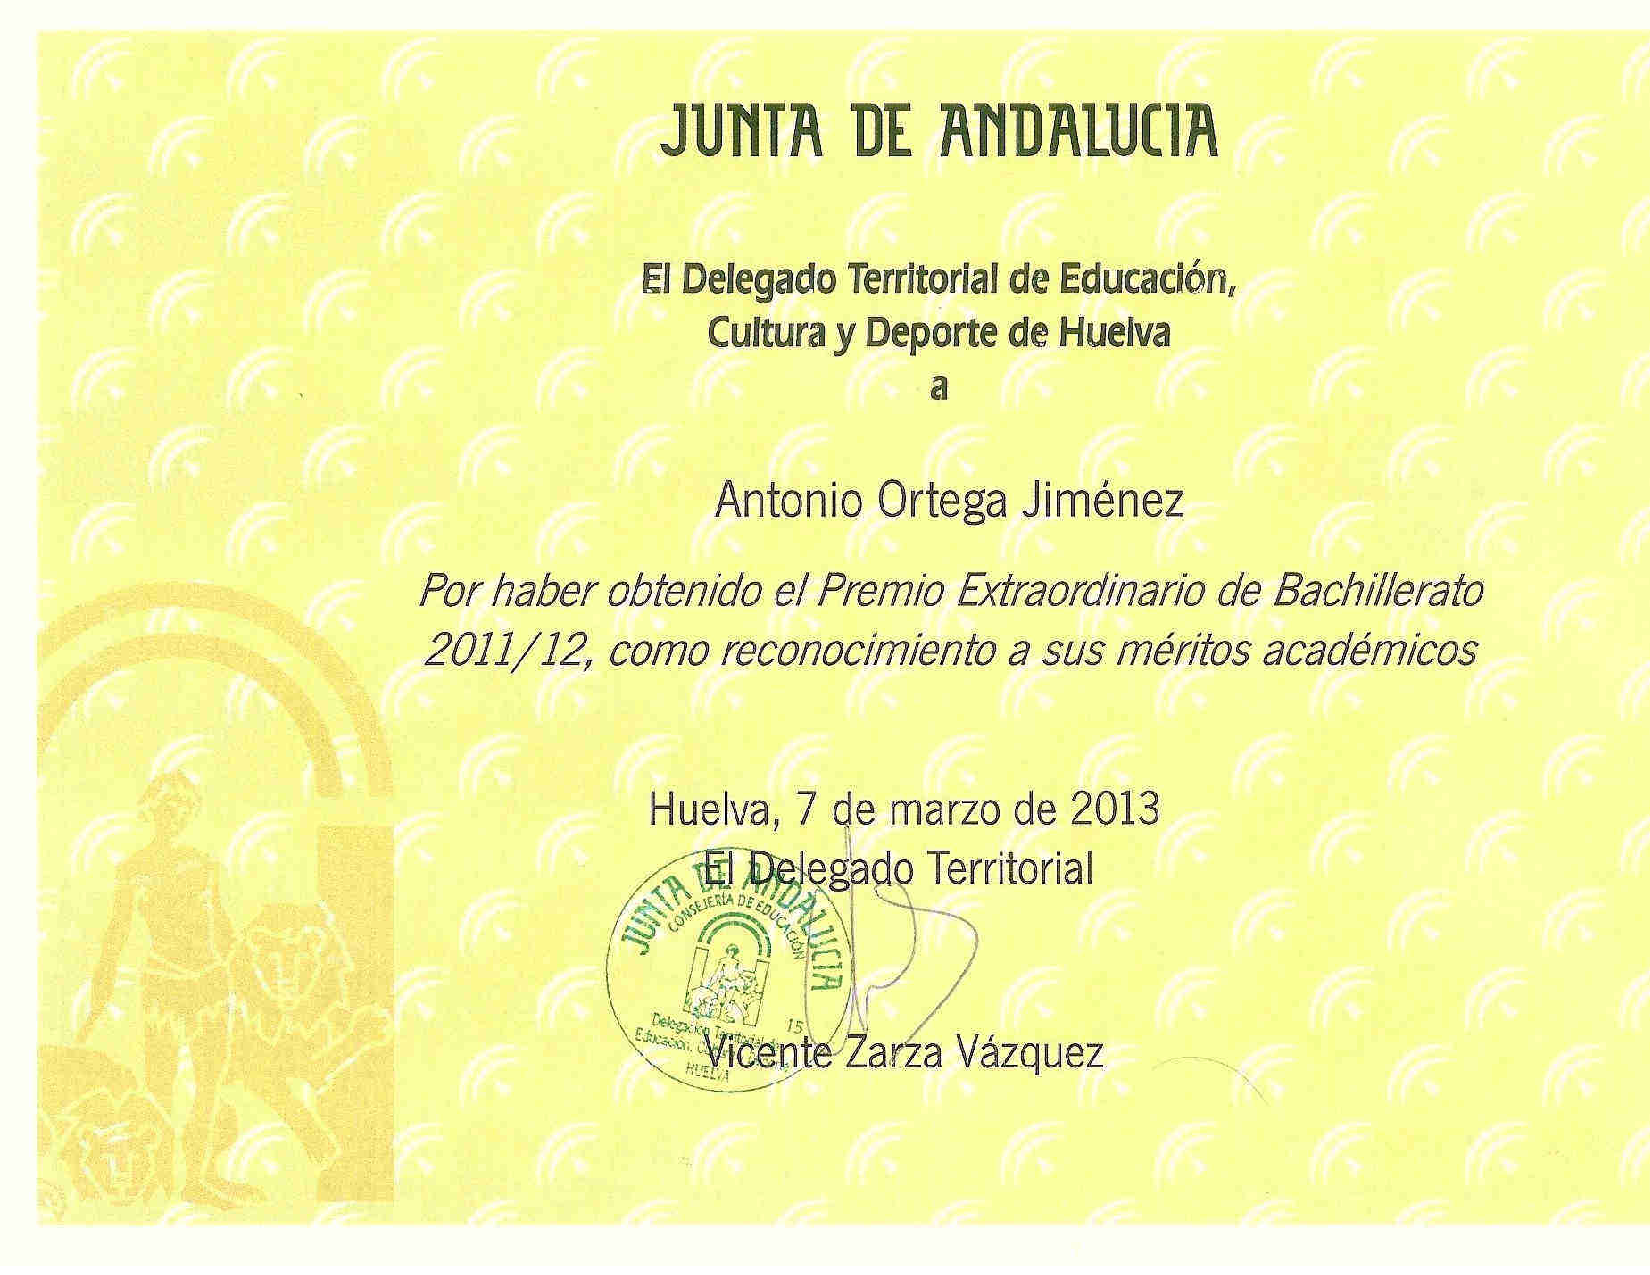
\includegraphics[scale=0.9]{./premio_extraordinario.pdf}
\end{landscape}
\restoregeometry
\clearpage


% Diploma del curso de bioinformatica en la complu
\thispagestyle{empty}

\newgeometry{margin=20pt, bottom=5pt}
\hypertarget{complu}{}
\begin{landscape}
\centering
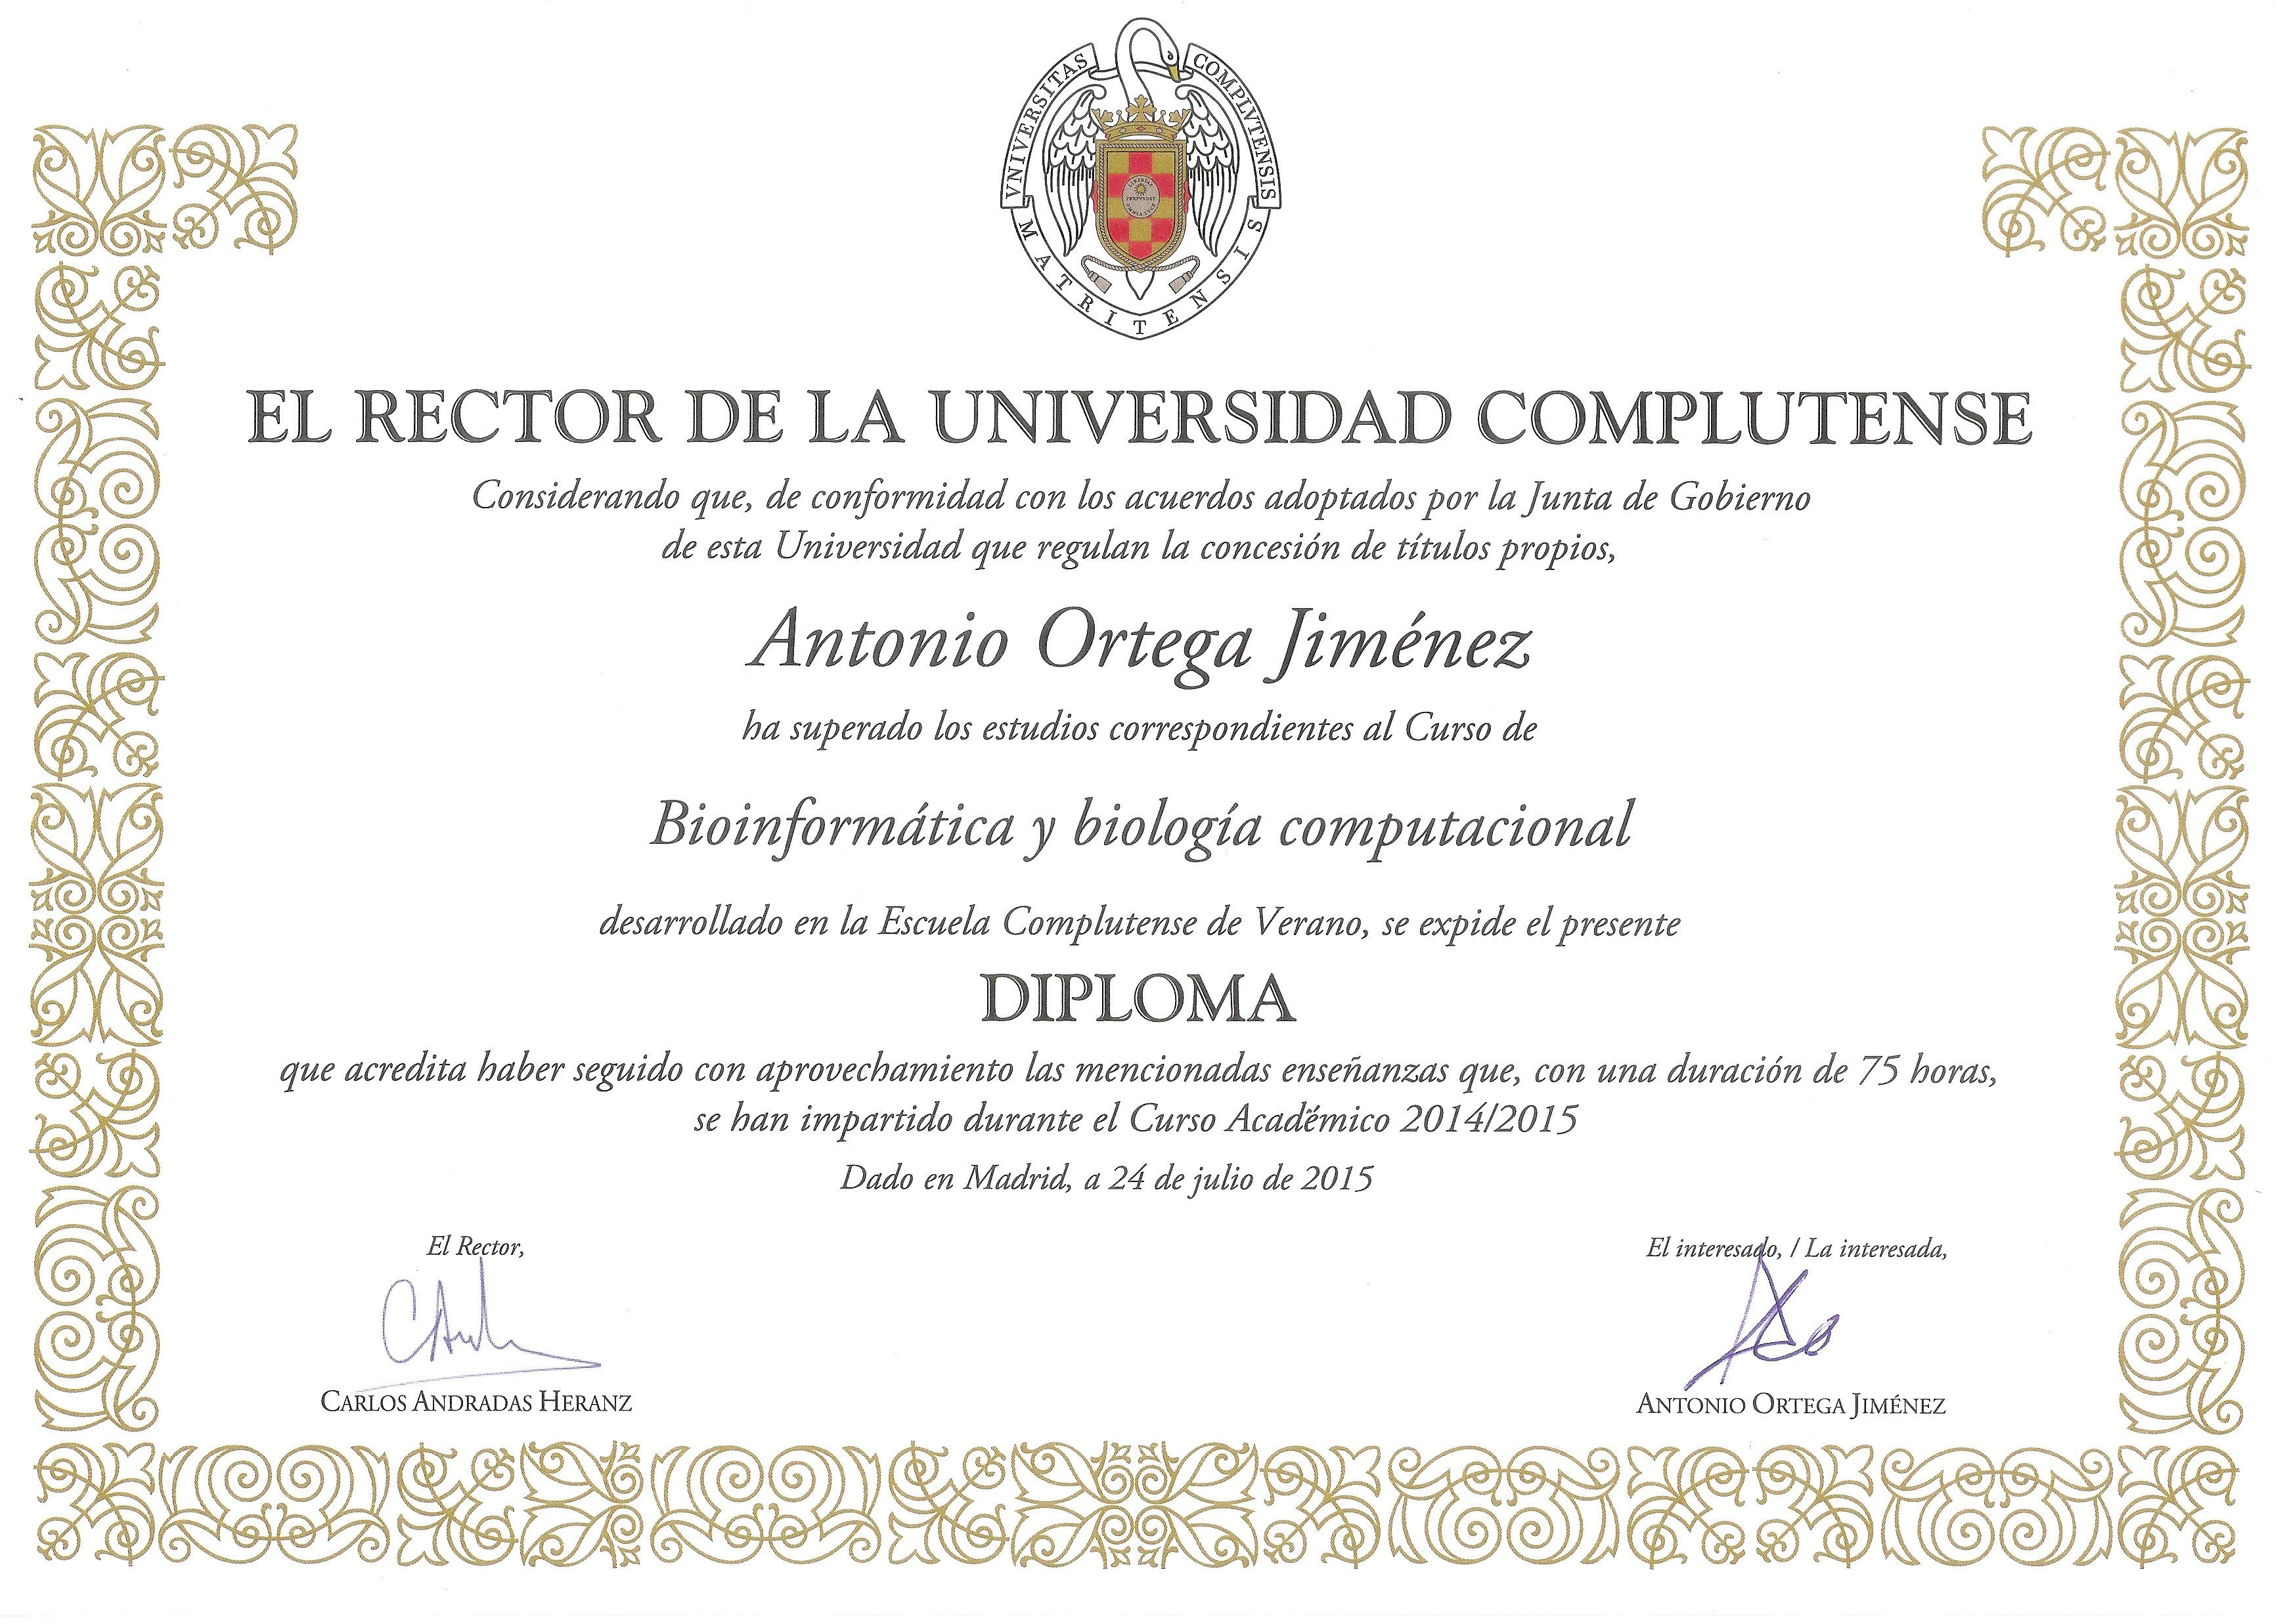
\includegraphics[scale=0.2]{./bioinformatica2.jpg}
\end{landscape}
\restoregeometry
\clearpage


\newgeometry{margin=20pt, bottom=5pt}
\hypertarget{ML-Coursera}{}
\begin{landscape}
\centering
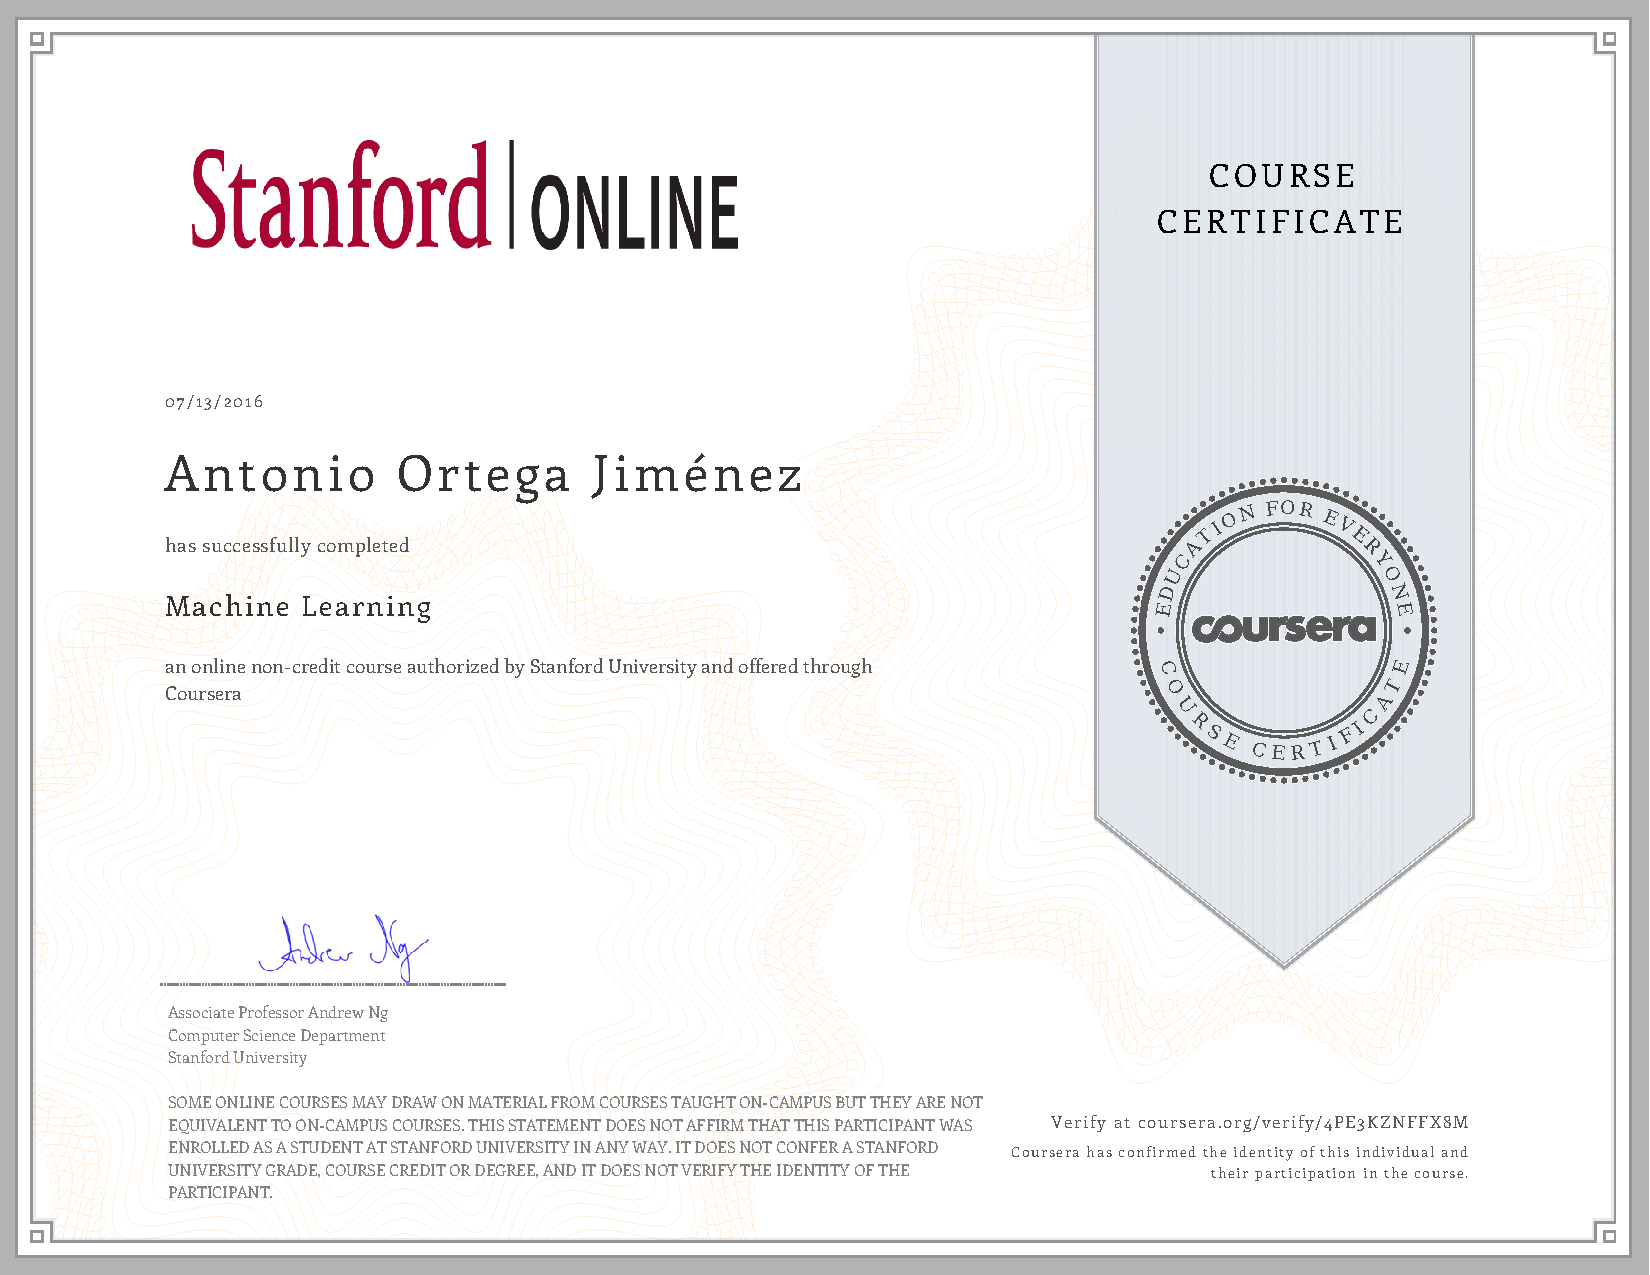
\includegraphics[width=\textwidth]{ML-Coursera.pdf}
\end{landscape}
\restoregeometry
\clearpage


%Expediente oficial en inglés
\hypertarget{exp-en}{}
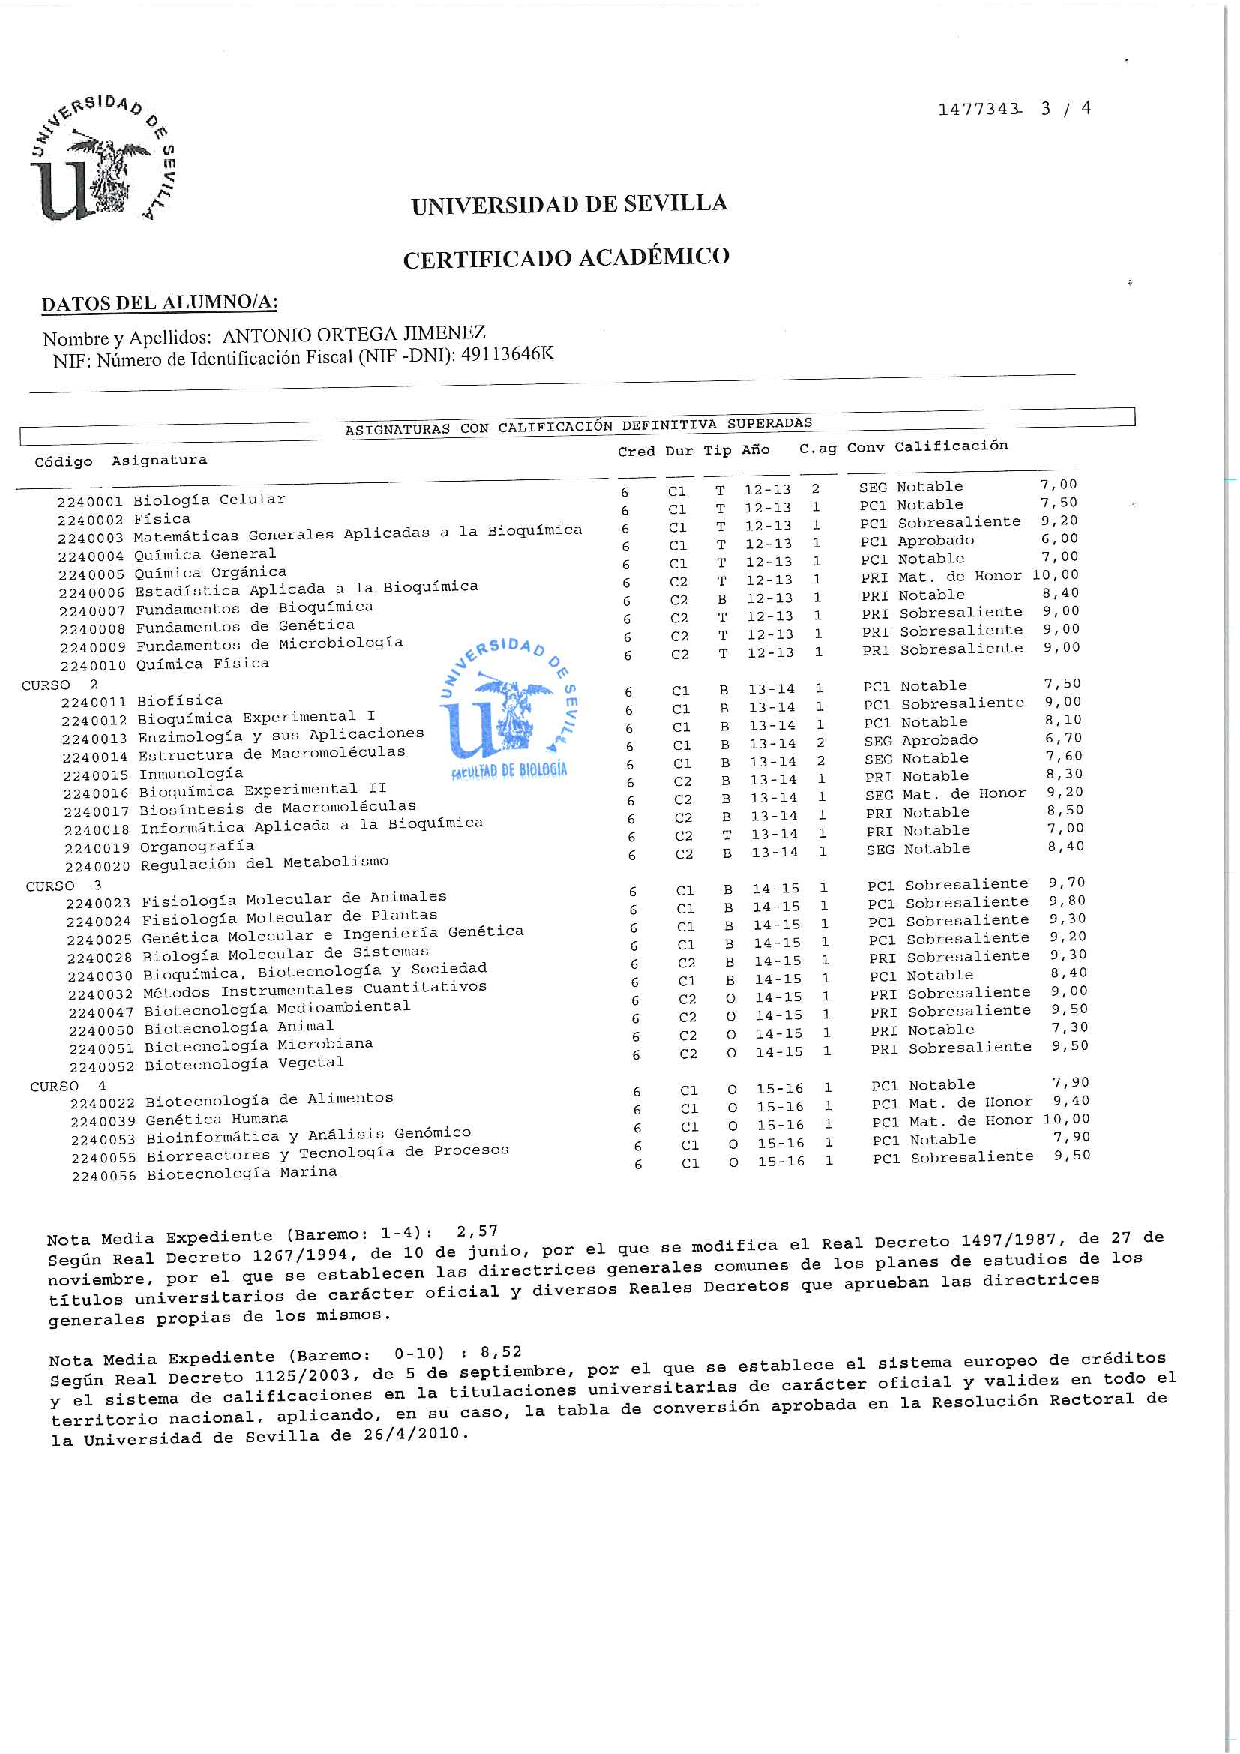
\includepdf[pages={1}]{certificado-es.pdf}
\clearpage


\hypertarget{cae}{}
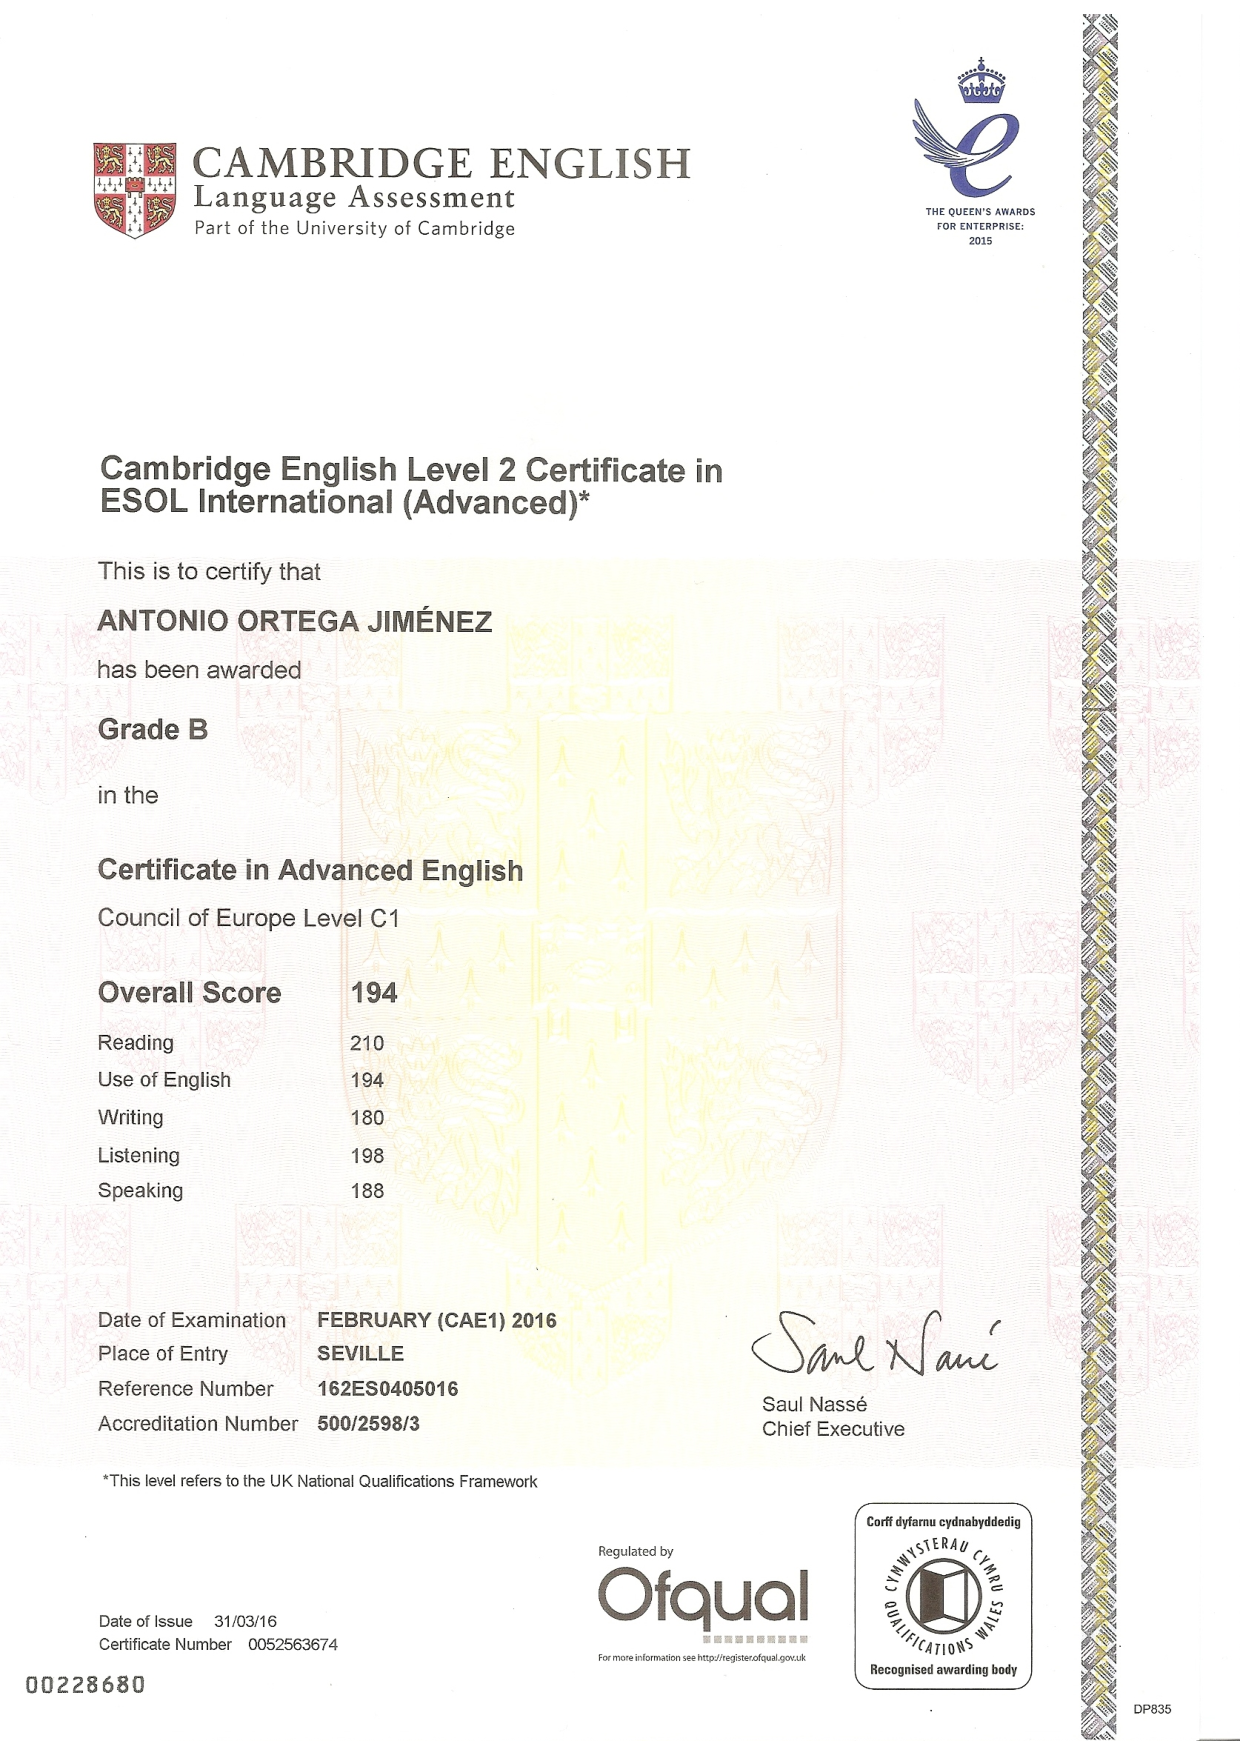
\includepdf{cae.pdf}
\clearpage



%Certificado DELF
%\thispagestyle{empty}
%\begin{landscape}
%\begin{figure}
%\hspace{-2.5 cm}
%\includegraphics[scale=0.3]{./delf.jpg}
%\end{figure}
%\end{landscape}
%\clearpage
\end{document}
